%===============================================================================
%===============================================================================
%
\clearpage
%
\section{Evaluation of time stepping widths}
%
 The center 30 nodes of a single fiber from the biceps is used to simulate activation for $t=30$ms with the Hodgkin-Huxley model.
 Different values for $dt_\text{0D}$, $dt_\text{1D}$ and $dt_\text{3D}$ are employed and the relative error per node to a reference solution is computed.

The used parameters are
\begin{equation*}
  \begin{array}{lll}
    c = \text{Conductivity/(Am*Cm)},\qquad \Omega = [0,50], \qquad t_\text{end}=50.
  \end{array}
\end{equation*}
The reference solution uses the following parameters:
\begin{table}[h!]
  \begin{center}
    \begin{tabular}{l|l}
      \textbf{Parameter} & \textbf{Value}\\
      \hline
      splitting timestep $dt_\text{3D}$ & $10^{-8}$\\
      timestep of diffusion term $dt_\text{1D}$ & $10^{-8}$\\
      timestep of ODEs $dt_\text{0D}$ & $10^{-8}$
    \end{tabular}
  \end{center}
  \caption{discretization parameters}
  \label{tab:table_monodomain2}
\end{table}
  
\subsection{Result summary}

\subsubsection{Evaluation of 0D time step width}
\vspace*{-0.2cm}
The following parameters are used: $dt_\text{1D}= 10^{-6}$, $dt_\text{3D} = dt_\text{0D}$.
\begin{figure}[h!]
  \centering%
  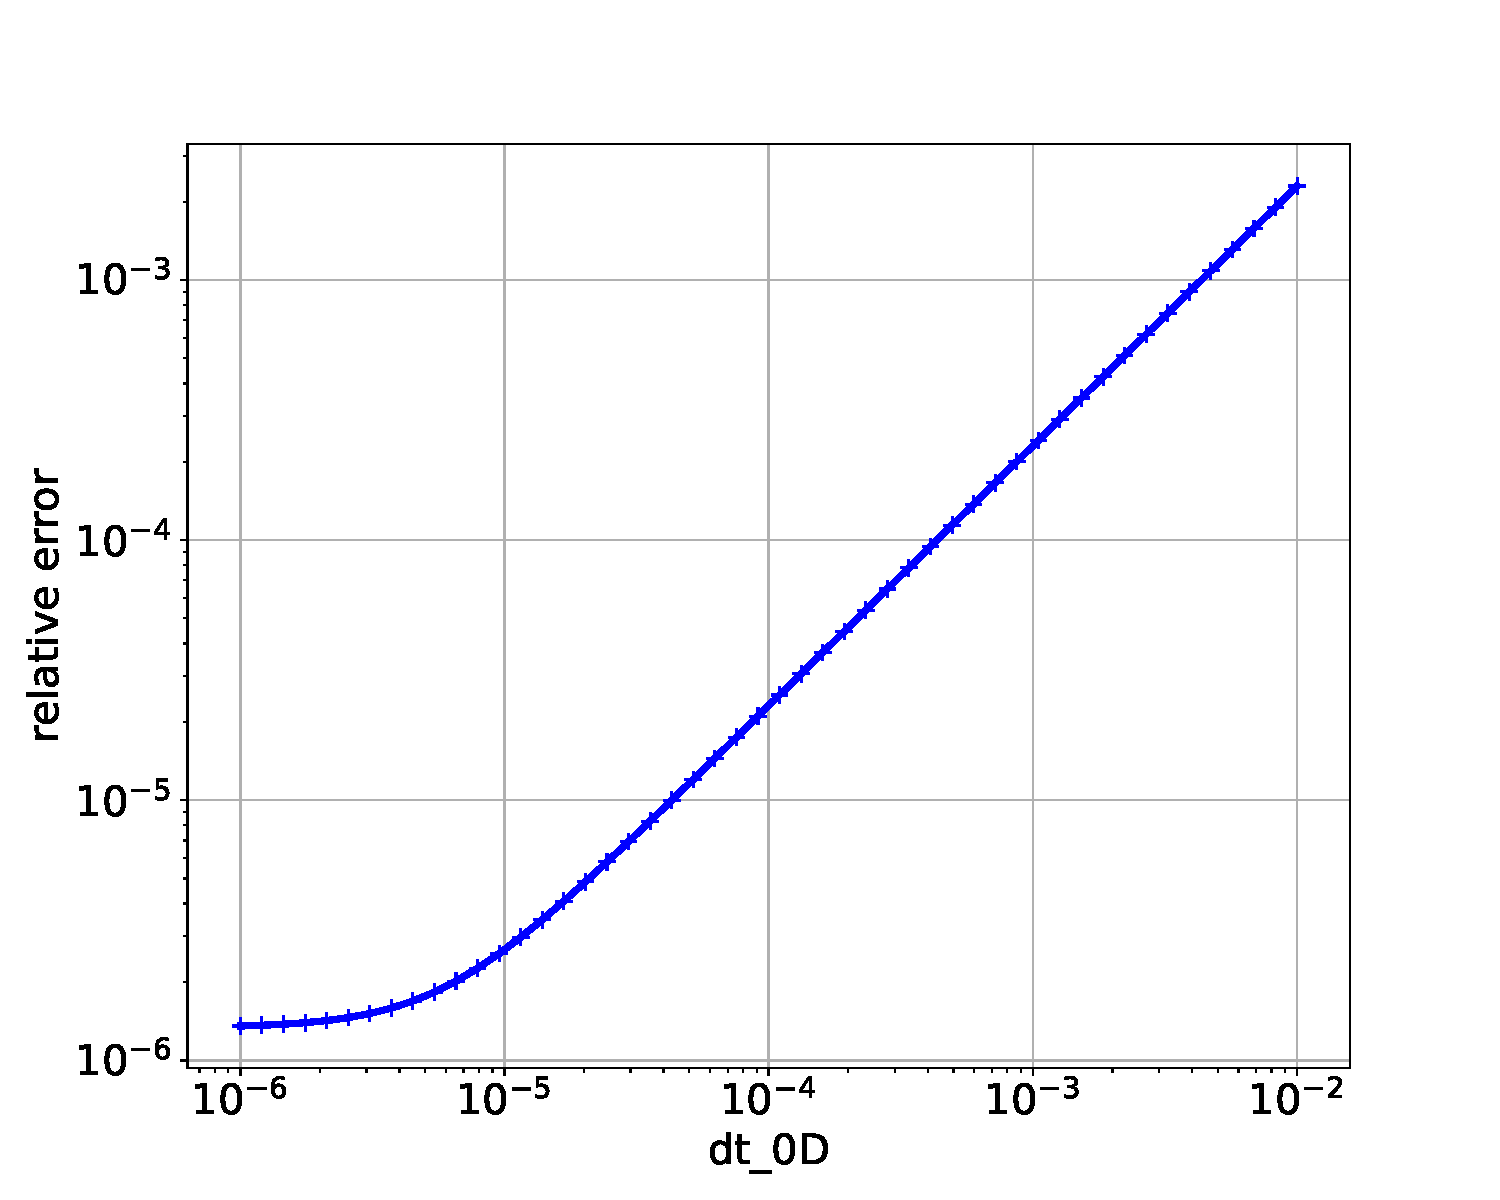
\includegraphics[height=0.7\textheight,width=\textwidth,keepaspectratio]{../tests/monodomain_timestep_widths/results/dt_0D.pdf}%
  \caption{0D time step width}
\end{figure} 

\subsubsection{Evaluation of 1D time step width}
\vspace*{-0.2cm}
The following parameters are used: $dt_\text{0D}= 10^{-6}$, $dt_\text{3D} = dt_\text{1D}$.
\begin{figure}[h!]
  \centering%
  \includegraphics[height=0.7\textheight,width=\textwidth,keepaspectratio]{../tests/monodomain_timestep_widths/results/dt_1D.pdf}%
  \caption{1D time step width}
\end{figure} 

\subsubsection{Evaluation of splitting scheme time step width}
\vspace*{-0.2cm}
The following parameters are used: $dt_\text{0D} = 10^{-6}$, $dt_\text{1D}= 10^{-6}$.
\begin{figure}[h!]
  \centering%
  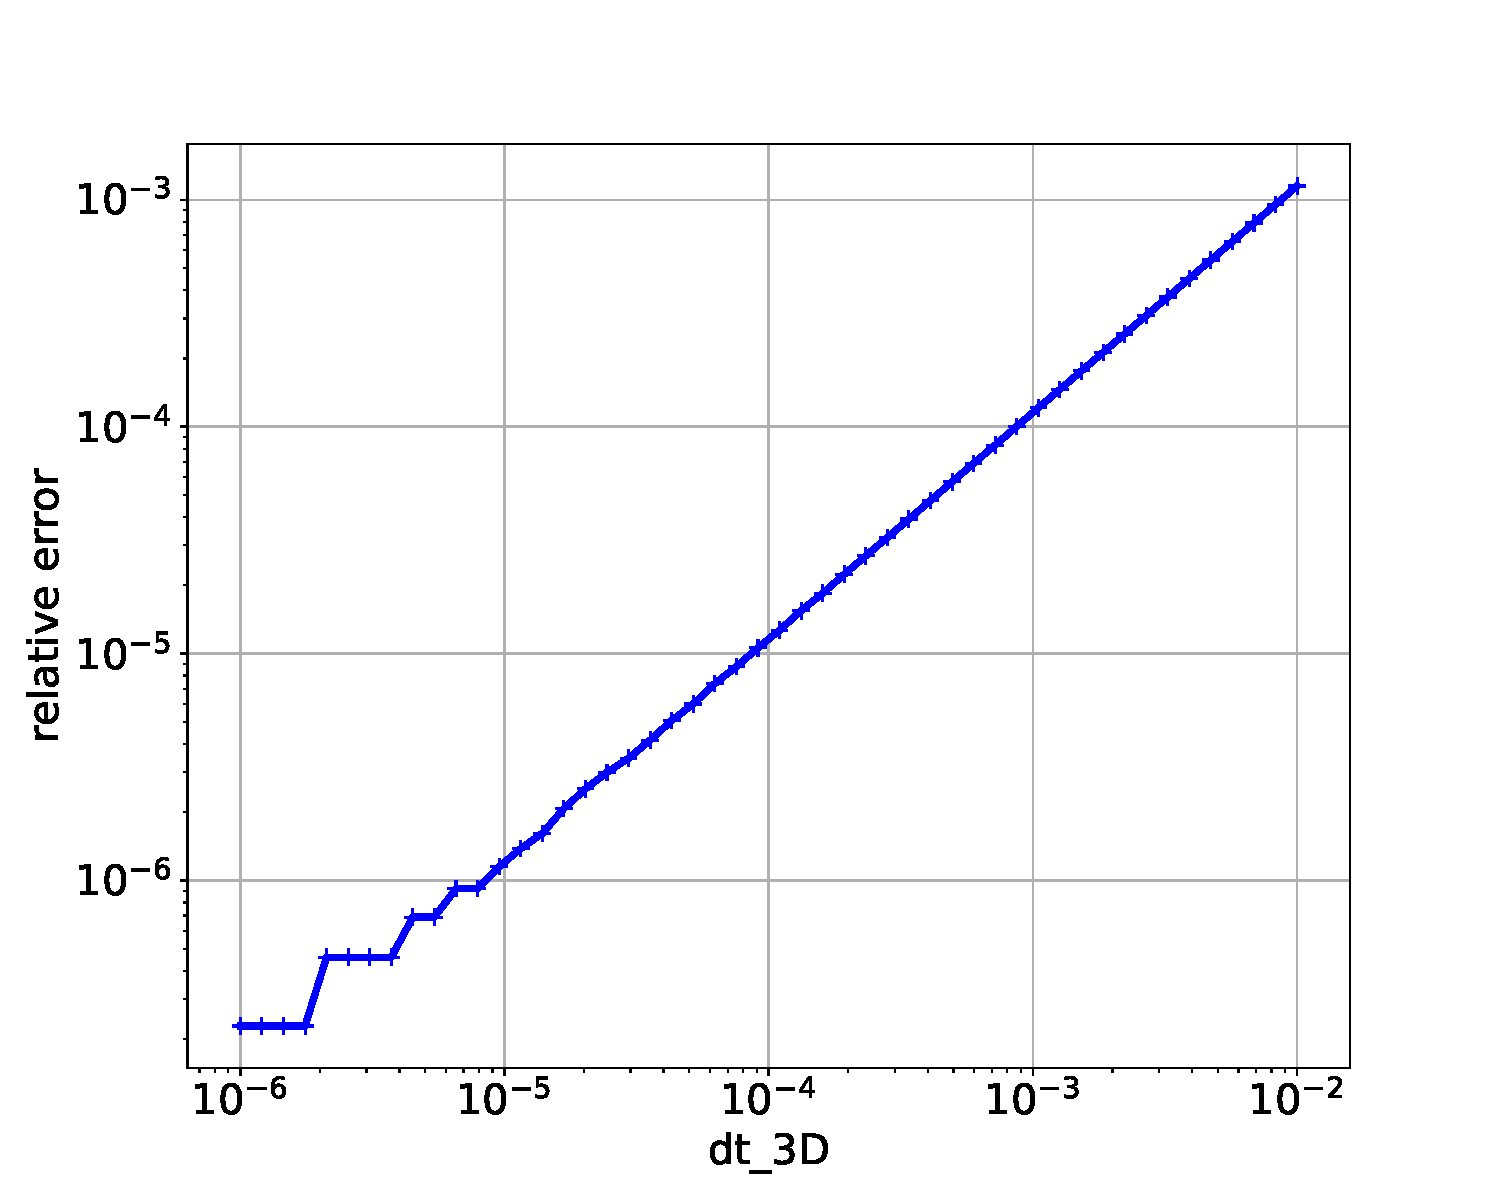
\includegraphics[height=0.7\textheight,width=\textwidth,keepaspectratio]{../tests/monodomain_timestep_widths/results/dt_3D.pdf}%
  \caption{splitting scheme time step width}
\end{figure} 

\subsubsection{Evaluation of splitting scheme time step width}
\vspace*{-0.2cm}
The following parameters are used: $dt_\text{0D}= 3\cdot 10^{-3}$, $dt_\text{1D} = 10^{-3}$.
\begin{figure}[h!]
  \centering%
  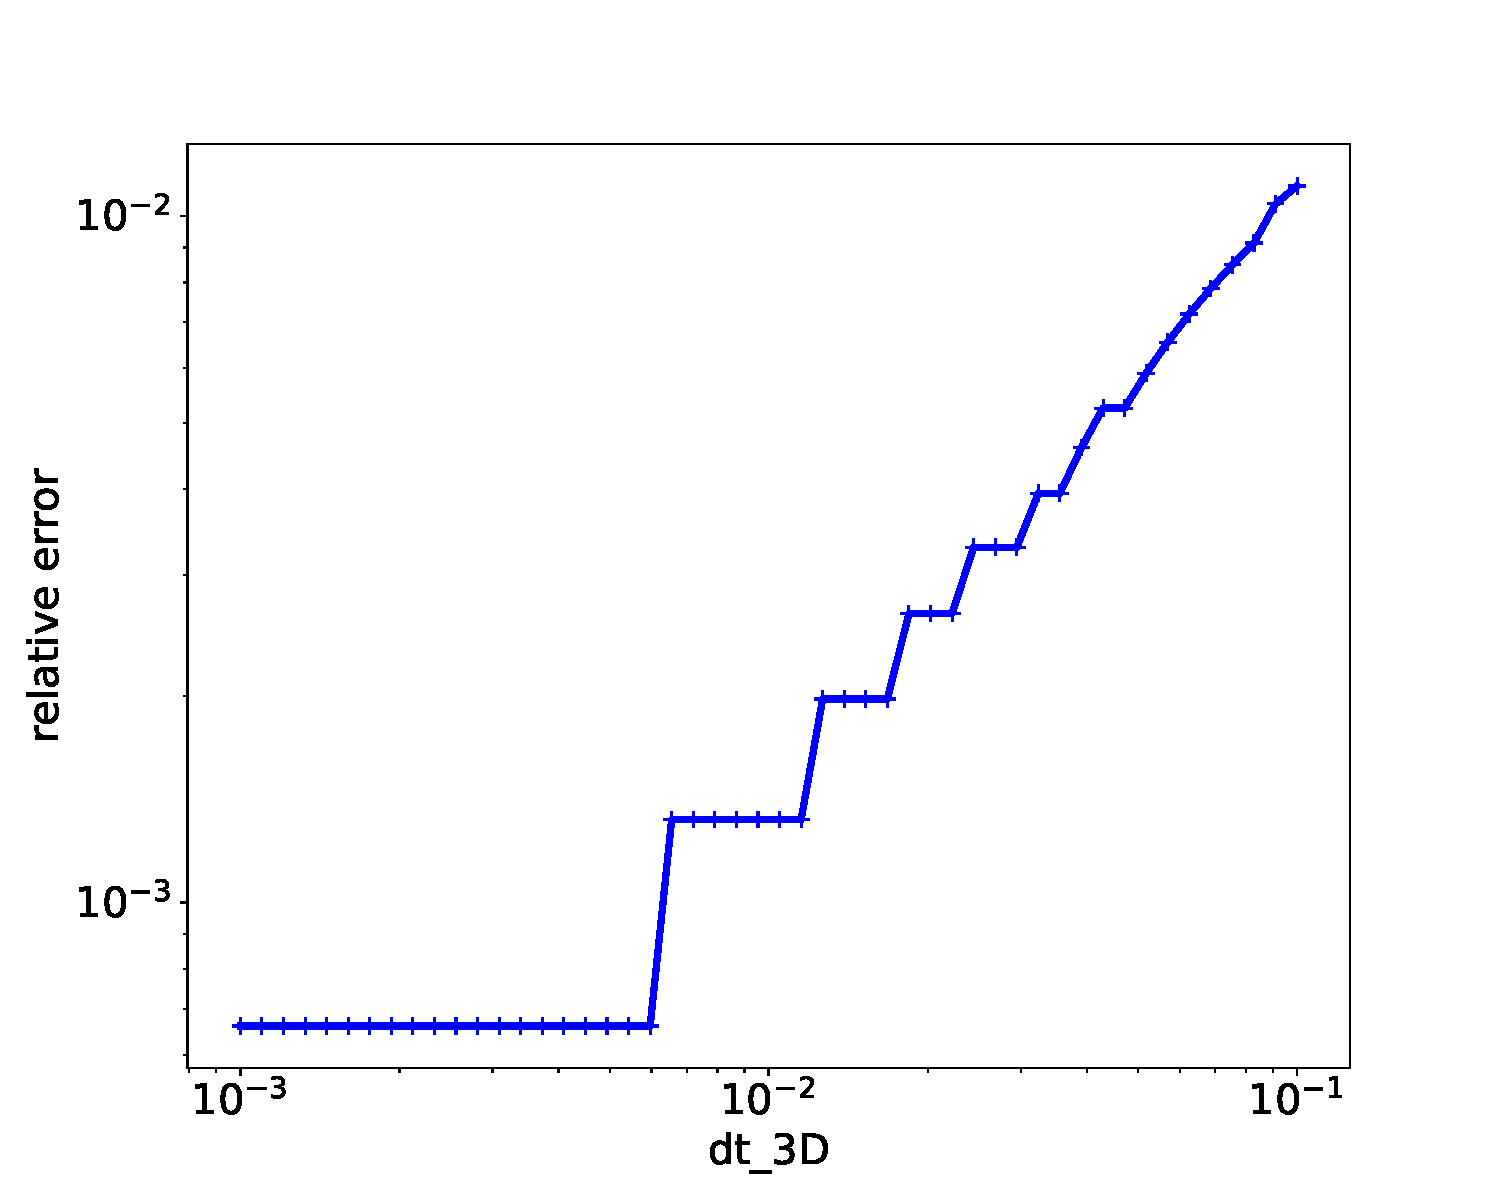
\includegraphics[height=0.7\textheight,width=\textwidth,keepaspectratio]{../tests/monodomain_timestep_widths/results/dt_3Db.pdf}%
  \caption{splitting scheme time step width}
\end{figure} 

\lstinputlisting[breaklines,basicstyle=\tiny]{../tests/multiple_fibers/results/log_recent_fiber_1.txt}
%
%===============================================================================
%===============================================================================
